%%%%%%%%%%%%%%%%%%%- HXN
\def\sode{11}
\def\tendethi{ĐỀ PHÁT TRIỂN MINH HOẠ 2025}
\begin{dethi}
 {\tendethi}
\end{dethi}
\caulc
\Opensolutionfile{ans}[ans/ans-HXN-\sode-T]
\begin{ex}%Câu 1
 Cho hàm số $ y=f(x)$ liên tục trên $\mathbb{R}$ và có bảng xét dấu của $f'(x)$ như sau:\\
\centerline{

\begin{tikzpicture}[>=stealth]
    \tkzTabInit[nocadre=true,lgt=1.2,espcl=2.5,deltacl=.5]
    {$x$/.7, $f'(x)$/1}
    {$-\infty$,$-2$,$0$,$2$,$+\infty$}
    \tkzTabLine{ , + , $0$ , - ,$0$,+,$0$,+, }
\end{tikzpicture}
}
 Hàm số $ y=f(x)$ có bao nhiêu điểm cực trị?
 \choice
 {$4$}
 {$3$}
 {\True $2$}
 {$1$}
\end{ex}
\begin{ex}%Câu 2
 Biết $\int\limits_1^3f(x)\mathrm{d}x=3$. Giá trị của $\int\limits_1^32f(x)\mathrm{d}x$ bằng
 \choice
 {$5$}
 {\True $6$}
 {$9$}
 {$\dfrac{3}{2}$}
\end{ex}
\begin{ex}%Câu 3
 Trong không gian $ Oxyz$, cho mặt phẳng $(P)$ đi qua điểm $ M\left(2;2;1\right)$ và có một vectơ pháp tuyến $\vec{n}=\left(5;2;-3\right)$. Phương trình mặt phẳng $(P)$là
 \choice
 {$5x+2y-3z-17=0$}
 {$2x+2y+z-11=0$}
 {\True $5x+2y-3z-11=0$}
 {$2x+2y+z-17=0$}
\end{ex}
\begin{ex}%Câu 4
 Nếu cấp số nhân $\left(u_n\right)$ có số hạng đầu $u_1=3$ và công bội $ q=3$ thì số hạng tổng quát $u_n$ của cấp số nhân đó bằng
 \choice
 {\True $3^{n}$}
 {$3^{n-1}$}
 {$3^{n+1}$}
 {$3+\left(n-1\right)\cdot 3$}
\end{ex}
\begin{ex}%Câu 5
 Tập nghiệm của bất phương trình $2^x\le 4$ là
 \choice
 {\True $\left(-\infty;2\right]$}
 {$\left[0;2\right]$}
 {$\left(-\infty;2\right)$}
 {$\left(0;2\right)$}
\end{ex}
\begin{ex}%Câu 6
 Cho hình chóp $S.ABCD$ có tất cả các cạnh bên và cạnh đáy bằng nhau và $ABCD$ là hình vuông tâm $O$. Khẳng định nào sau đây là khẳng định đúng?
 \choice
 {$SA\perp\left(ABCD\right)$}
 {\True $SO\perp\left(ABCD\right)$}
 {$AB\perp\left(SBC\right)$}
 {$AC\perp\left(SBC\right)$}
\end{ex}
\begin{ex}%Câu 7
 Phát biểu nào sau đây là đúng?
 \choice
 {$\int\dfrac{1}{x}\mathrm{\,d}x=\left| x\right|+\text{C}$}
 {\True $\int\dfrac{1}{x}\mathrm{\,d}x=\text{ln}\left| x\right|+C$}
 {$\int\text{ln}x\mathrm{\,d}x=x+C$}
 {$\int\text{ln}\left| x\right|\mathrm{\,d}x=\text{ln}x+C$}
\end{ex}
\begin{ex}%Câu 8
\immini
{
     Cho hàm số $y=f(x)$ có đồ thị như hình dưới đây.
 Đường tiệm cận xiên của đồ thị hàm số đã cho là đường thẳng 
 \choice
 {$y=x-1$}
 {\True $y=-x-1$}
 {$y=x+1$}
 {$y=-x+1$}
}
{
    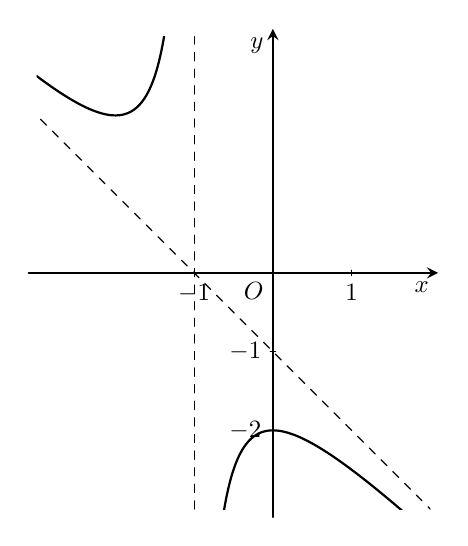
\begin{tikzpicture}[line join=round, line cap=round,>=stealth,thick]
        \tikzset{every node/.style={scale=0.9}}
        \draw[->] (-3.1,0)--(2.1,0) node[below left] {$x$};
        \draw[->] (0,-3.1)--(0,3.1) node[below left] {$y$};
        \draw (0,0) node [below left] {$O$};
        \foreach \x/\nx in {-1/-1,1/1}
        \draw[thin] (\x,1pt)--(\x,-1pt) node [below] {$\nx$};
        \foreach \y/\ny in {-2/-2,-1/-1}
        \draw[thin] (1pt,\y)--(-1pt,\y) node [left] {$\ny$};
        \draw[dashed,thin] (-0.99,-3)--(-0.99,3);
        \begin{scope}
            \clip (-3,-3) rectangle (2,3);
            \draw[samples=200,domain=-3:-1.01,smooth,variable=\x] plot (\x,{(-1*((\x)^2)+-2*(\x)+-2)/(1*(\x)+1)});
            \draw[samples=200,domain=-0.99:3,smooth,variable=\x] plot (\x,{(-1*((\x)^2)+-2*(\x)+-2)/(1*(\x)+1)});
            \draw[dashed,thin] (-3.1,2.1)--(3.1,-4.1);
        \end{scope}
    \end{tikzpicture}
}
\end{ex}
\begin{ex}%Câu 9
\immini
{
     Cho hàm số $f(x)$ có đồ thị như hình vẽ bên. Giá trị nhỏ nhất của hàm số $f(x)$ trên đoạn $\left[-2;2\right]$ bằng
 \choice
 {$-2$}
 {$-1$}
 {\True $ 0$}
 {$ 1$}
}
{
    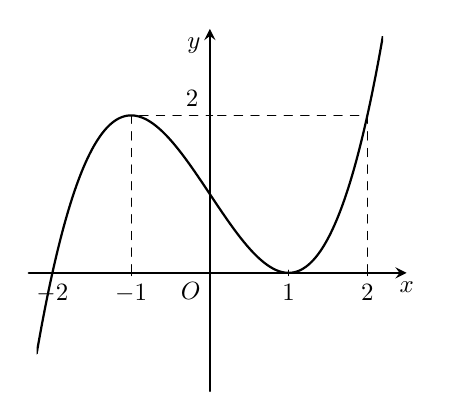
\begin{tikzpicture}[line join=round, line cap=round,>=stealth,thick]
        \tikzset{every node/.style={scale=0.9}}
        \draw[->] (-2.3,0)--(2.5,0) node[below] {$x$};
        \draw[->] (0,-1.5)--(0,3.1) node[below left] {$y$};
        \draw (0,0) node [below left] {$O$};
        \foreach \x/\nx in {-2/-2,-1/-1,1/1,2/2}
        \draw[thin] (\x,1pt)--(\x,-1pt) node [below] {$\nx$};
        \foreach \y/\ny in {2/2}
        \draw[thin] (1pt,\y)--(-1pt,\y) node [above left] {$\ny$};
        \draw[dashed,thin](-1,0)--(-1,2)--(0,2);
        \draw[dashed,thin](2,0)--(2,2)--(0,2);
        \begin{scope}
            \clip (-2.2,-1.5) rectangle (2.2,3);
            \draw[samples=200,domain=-2.2:2.2,smooth,variable=\x] plot (\x,{1/2*((\x)^3)+0*((\x)^2)+-3/2*(\x)+1});
        \end{scope}
    \end{tikzpicture}
}
\end{ex}
\begin{ex}%Câu 10
 Bạn An rất thích nhảy hiện đại. Thời gian tập nhảy mỗi ngày của bạn An được thống kê lại ở bảng sau:\\
 \centerline{
 \begin{tblr}{
         colspec = {Q[l] *{5}{Q[c]}},hlines,vlines
     }
     Thời gian (phút) & [20;25) & [25;30) & [30;35) & [35;40) & [40;45) \\
     Số ngày          & 6       & 6       & 4       & 1       & 1       \\
 \end{tblr}
 }
 Độ lệch chuẩn của mẫu số liệu ghép nhóm có giá trị gần nhất với giá trị nào dưới đây?
 \choice
 {$31{,}25$}
 {$31{,}26$}
 {$5{,}4$}
 {\True $5{,}6$}
\end{ex}
\begin{ex}%Câu 11
 Trong không gian $Oxyz$, điểm nào dưới đây thuộc đường thẳng $ d:\heva{& x=1-t\\& y=5+t\\& z=2+3t}$ ?
 \choice
 {$Q\left(-1;1;3\right)$}
 {$P\left(1;2;5\right)$}
 {$M\left(1;1;3\right)$}
 {\True $N\left(1;5;2\right)$}
\end{ex}
\begin{ex}%Câu 12
\immini
{
     Cho hình lập phương $ABCD.A'B'C'D'$(tham khảo hình bên). Giá trị $\sin$ của góc giữa đường thẳng $ AC'$ và mặt phẳng $\left(ABCD\right)$ bằng
 \choice
 {\True $\dfrac{\sqrt{3}}{3}$}
 {$\dfrac{\sqrt{2}}{2}$}
 {$\dfrac{\sqrt{3}}{2}$}
 {$\dfrac{\sqrt{6}}{3}$}
}
{
    \begin{tikzpicture}[line cap=round,line join=round, >=stealth,scale=1]
        \def \a{-1.5} \def \b{-1}\def \c{4} \def \h{3}
        \path (0,0)coordinate(A) 
        +(\a,\b)coordinate(B)
        +(\c,0)coordinate(D)
        ($(B)+(D)-(A)$)coordinate(C)
        +(0,\h) coordinate(C')
        ($(B)+(C')-(C)$)coordinate(B')
        ($(A)+(C')-(C)$)coordinate(A')
        ($(D)+(C')-(C)$)coordinate(D');
        \draw [dashed] (A)--(B)(D)--(A)--(A');
        \draw (B')--(B)--(C)(B')--(C')--(C)--(D)--(D')--(A')--(B')(C')--(D');
        \foreach \x/\g in {A/135,B/-135,C/-45,D/0,A'/135,B'/180,C'/-20,D'/0}\fill[red] (\x) circle (1pt)+(\g:3mm) node[black]{$\x$};
    \end{tikzpicture}
}
 \end{ex}
\Closesolutionfile{ans}
\cauds
\Opensolutionfile{ans}[ans/ans-HXN-\sode-TF]
\begin{ex}%Câu 13
\immini
{
    Công thức $\log x=11{,}8+1{,}5M$ cho biết mối liên hệ giữa năng lượng $x$ tạo ra (tính theo erg, $1$ erg tương đương $10^{-7}$ jun) với độ lớn $M$ theo thang Richter của một trận động đất
     \choiceTF
    {\True Nếu năng lượng được tạo ra là $ 6{,}3\cdot 10^{14}$ erg thì trận động đất phải có độ lớn bằng 2 độ Richter (làm tròn kết quả đến hàng đơn vị)}
    {Trận động đất có độ lớn $3$ độ Richter tạo ra năng lượng bằng $\left(10^{163}-10^{10}\right)$ erg}
    {\True Trận động đất có độ lớn $5$ độ Richter tạo ra năng lượng gấp $1000$ lần so với trận động đất có độ lớn $3$ độ Richter}
    {\True Người ta ước lượng rằng một trận động đất có độ lớn khoảng từ $4$ đến $6$ độ Richter thì năng lượng do trận động đất đó tạo ra nằm trong khoảng từ $10^{17,8}$erg đến $10^{20{,}8}$ erg}
}
{
    \includegraphics[width=5cm]{img/HXN-11-13}
}
\loigiai{
    \begin{itemchoice}
        \itemch 
        Ta có $x=6{,}3\cdot 10^{14} \Rightarrow M=\dfrac{\log \left(6{,}3\cdot 10^{14}\right)-11{,}8}{1{,}5}\approx 2$ độ Richter.
        \itemch Ta có $M=3 \Rightarrow \log x=11{,}8+1{,}5\cdot 3\Rightarrow x=10^{16{,}3}$ erg. 
        \itemch Gọi $x_3$, $x_5$ lần lượt là năng lượng tạo ra bởi các trận động đất có độ lớn 3 và 5 độ Richter.
        Ta có hệ phương trình $\heva{& \log x_3=11{,}8+1{,}5\cdot 3&&(1) \\& \log x_5=11{,}8+1{,}5\cdot 5&&(2)} $\\
        Lấy $(1)-(2)$ ta được $\log x_3-\log x_5=-3\Rightarrow \log \dfrac{x_3}{x_5}=-3 \Rightarrow \dfrac{x_3}{x_5}=\dfrac{1}{1\,000}\Rightarrow x_5=1\,000x_3$.\\
        Vậy trận động đất có độ lớn $5$ độ Richter tạo ra năng lượng gấp $1\,000$ lần so với trận động đất có độ lớn 3 độ Richter.
        \itemch Gọi $x_4$, $x_6$ lần lượt là năng lượng tạo ra bởi các trận động đất có độ lớn 4 và 6 độ Richter. \\
        Ta có $\heva{& \log x_4=11{,}8+1{,}5\cdot 4\\& \log x_6=11{,}8+1{,}5\cdot 6} \Leftrightarrow \heva{& \log x_4=17{,}8 \\& \log x_6=20{,}8 } \Leftrightarrow \heva{& x_4=10^{17{,}8} \\& x_6=10^{20{,}8}.}$ \\
        Vậy một trận động đất có độ lớn khoảng từ $4$ đến $6$ độ Richter thì năng lượng mà nó tạo ra nằm trong khoảng từ $10^{17{,}8}$erg đến $10^{20{,}8}$erg.
    \end{itemchoice}
}
\end{ex}
\begin{ex}%Câu 14
\immini
{
    Tại một thành phố du lịch vào những ngày tháng $6$, người ta luôn chứng kiến trời nắng hoặc trời mưa (mỗi ngày có thể trời nắng xong đến mưa và ngược lại). Người ta biết được có $\dfrac{2}{3}$ số ngày trong tháng là có nắng, có $\dfrac{5}{6}$ số ngày trong tháng là có mưa. Nếu hôm nào bầu trời tại thành phố chỉ có mưa thì khả năng kẹt xe gấp đôi khả năng không kẹt xe; nếu hôm nào bầu trời chỉ có nắng thì chắc chắn thành phố không xảy ra kẹt xe; những ngày trời vừa có nắng vừa có mưa thì khả năng kẹt xe là $30\%$.
}
{
    \includegraphics[width=5cm]{img/HXN-11-14}
}
 \choiceTF
 {\True Nếu du khách đến thành phố vào ngày chỉ có mưa thì khả năng kẹt xe bằng $\dfrac{2}{3}$}
 {Trong tháng 6, có $10$ ngày mà thành phố vừa có mưa vừa có nắng}
 {Một du khách đang cân nhắc sẽ đến thành phố vào một ngày tháng 6, xác suất du khách gặp cảnh kẹt xe bằng $ 0{,}32$ (làm tròn đến hàng phần trăm)}
 {Sau khi du khách đến nơi thì hôm ấy xảy ra kẹt xe thật, xác suất để thành phố vừa có nắng, vừa có mưa bằng $0{,}3$ (làm tròn đến hàng phần chục)}
 \loigiai{
     \begin{itemchoice}
         \itemch Vào ngày chỉ có mưa, khả năng kẹt xe gấp đôi khả năng không kẹt xe nên khả năng kẹt xe tại thành phố là $\dfrac{2}{3}$ và khả năng không kẹt xe là $\dfrac{1}{3}$.
         \itemch Trong tháng sẽ có $\dfrac{2}{3}+\dfrac{5}{6}-1=\dfrac{1}{2}$ số ngày vừa có nắng vừa có mưa, có $\dfrac{2}{3}-\dfrac{1}{2}=\dfrac{1}{6}$ số ngày chỉ có nắng và có $\dfrac{5}{6}-\dfrac{1}{2}=\dfrac{1}{3}$ số ngày chỉ có mưa.\\
         Số ngày trong tháng vừa có mưa vừa có nắng tại thành phố là $\left(\dfrac{2}{3}+\dfrac{5}{6}-1\right)\cdot 30=15$ (ngày).
         \itemch Gọi A là biến cố: \lq\lq Ngày có nắng tại thành phố\rq\rq, B là biến cố: \lq\lq Ngày có mưa tại thành phố\rq\rq và C là biến cố \lq\lq Ngày có sự cố kẹt xe xảy ra tại thành phố\rq\rq. Ta tham khảo sơ đồ bên cạnh.\\
         \centerline{
             \includegraphics[width=6cm]{img/HXN-11-14-LG}
         }
         Xác suất kẹt xe xảy ra là $P(C)=\dfrac{1}{6}\cdot 0+\dfrac{1}{2}\cdot \dfrac{3}{10}+\dfrac{1}{3}\cdot \dfrac{2}{3}=\dfrac{67}{180}\approx 0{,}37$.
         \itemch Ta có: $P\left(AB|C\right)=\dfrac{P(ABC)}{P(C)}=\dfrac{\dfrac{1}{2}\cdot \dfrac{3}{10}}{\dfrac{67}{180}}=\dfrac{27}{67}\approx 0{,}4$.
     \end{itemchoice}
 }
\end{ex}
\begin{ex}%Câu 15
Một khối gỗ có dạng khối nón có bán kính đáy $r=30$ cm, chiều cao $h=120$ cm. Người thợ mộc tìm cách chế tác khối gỗ đó thành một khúc gỗ có dạng khối trụ như hình vẽ.\\
\centerline{
\includegraphics[width=.5\textwidth]{img/HXN-11-15}
}
 \choiceTF
 {\True Thể tích khối gỗ ban đầu bằng $36\,000\pi {cm^3}$}
 {\True Nếu người thợ mộc muốn tạo ra khối gỗ hình trụ có chiều cao bằng nửa khối gỗ ban đầu thì khối gỗ mới tạo ra có thể tích $ 13500\pi$}
 {\True Nếu người thợ mộc muốn tạo ra khối gỗ hình trụ có bán kính đáy bằng $\dfrac{2}{3}$ bán kính khối gỗ hình nón thì phần gỗ phải bỏ đi có thể tích bằng $ 20000\pi {cm^3}$}
 {\True Thể tích lớn nhất của khối gỗ hình trụ bằng $ 0,016\pi \,m^3$}
 \loigiai{
     \begin{itemchoice}
         \itemch Thể tích khối gỗ hình nón là $V=\dfrac{1}{3}\pi r^2h=\dfrac{1}{3}\pi \cdot 30^2\cdot 120=36\,000\pi \,cm^3$.
         \itemch Xét một nửa thiết diện qua trục của hình nón là tam giác SAB (tham khảo hình vẽ).\\
         \centerline{
             \includegraphics[width=5cm]{img/HXN-11-15-LG}
         }
         Các tam giác $SMN$ và $SAB$ đồng dạng (có $\widehat{S}$ chung, $\widehat{SMN}=\widehat{SAB}=90^0$),\\
         ta có $\dfrac{MN}{AB}=\dfrac{SM}{SA}\Leftrightarrow \dfrac{MN}{30}=\dfrac{1}{2}\Rightarrow MN=15\,cm$.\\
         Khối gỗ hình trụ mới được tạo thành có bán kính đáy $15\,cm$, chiều cao $60\,cm$ nên có thể tích $\pi \cdot 15^2\cdot 60=13\,500\pi \,cm^3$.
         \itemch Bán kính đáy khối gỗ hình trụ là $\dfrac{2}{3}\cdot 30=20\,cm$.\\
         Các tam giác $SMN$ và $SAB$ đồng dạng (có $\widehat{S}$ chung, $\widehat{SMN}=\widehat{SAB}=90^0$),\\
         ta có $\dfrac{MN}{AB}=\dfrac{SM}{SA}\Leftrightarrow \dfrac{2}{3}=\dfrac{SM}{120}\Rightarrow SM=80\,cm\Rightarrow AM=40\,cm$.\\
         Thể tích khối gỗ phải bỏ đi là $36\,000\pi -\pi \cdot 20^2\cdot 40=20\,000\pi \,cm^3$.
         \itemch Đặt $AM=x\,\,(cm)$ $(0<x<120)$. \\
         Ta có $\dfrac{MN}{AB}=\dfrac{SM}{SA}\Leftrightarrow \dfrac{MN}{30}=\dfrac{120-x}{120}\Rightarrow MN=30-\dfrac{x}{4}$.\\
         Vậy khối trụ mới được tạo thành có bán kính $MN=30-\dfrac{x}{4}$, đường cao $AM=x$ nên có thể tích: 
         $$V=\pi \left(30-\dfrac{x}{4}\right)^2x=\pi \cdot \left(30-\dfrac{x}{4}\right)\cdot \left(30-\dfrac{x}{4}\right)\cdot \dfrac{x}{2}\cdot 2$$
         Xét hàm số $V(x)=\pi \left(30-\dfrac{x}{4}\right)^2x=\pi \left(900x-15x^2+\dfrac{1}{16}x^3\right)$  với $0<x<120$.\\
         Ta có $V'(x)=\pi \left(900-30x+\dfrac{3x^2}{16}\right)=0 \Leftrightarrow \hoac{& x=120 &&\text{(loại)} \\& x=40 &&\text{(nhận)}}$.\\
         Bảng biến thiên:\\
         
\begin{tikzpicture}[>=stealth]
             \tkzTabInit[nocadre=false,lgt=1.2,espcl=2.5,deltacl=0.5]{$x$/.7 ,$V'(x)$/.7,$V(x)$/2}
             {$0$ , $40$ , $120$}
             \tkzTabLine{ , + , $0$ , - , }
             \tkzTabVar{-/$1$ , +/$16\,000\pi$ , -/$5$}
         \end{tikzpicture}\\
         Dễ thấy $V_{\max}=16\,000\pi \,cm^3=0{,}016\pi \,m^3$.
     \end{itemchoice}
 }
\end{ex}
\begin{ex}%Câu 16
\immini
{
    Trong không gian với hệ tọa độ $Oxyz$, đơn vị trên mỗi trục tọa độ là $km$, NASA đang thiết kế một trạm vũ trụ hình cầu có tâm đặt tại điểm $ O(0;0;0)$ và bán kính $R=10$ km. Một con tàu vũ trụ di chuyển với tốc độ $ 27000$ km/h theo quỹ đạo là một đường thẳng qua điểm $ A(6;8;0)$ và có vectơ chỉ phương $\vec{u}=(2;2;-1)$
}
{
    \includegraphics[width=5cm]{img/HXN-11-16}
}
 \choiceTF
 {Điểm $ A(6;8;0)$ nằm bên trong trạm vũ trụ hình cầu}
 {\True Phương trình quỹ đạo di chuyển của tàu vũ trụ là $\Delta \colon \heva{& x=6+2t\\& y=8+2t\\& z=-t}$ ($t$ là tham số)}
 {Khoảng cách từ tâm của trạm vũ trụ đến đường thẳng quỹ đạo tàu vũ trụ là $3{,}8$ km (làm tròn đến hàng phần chục, đơn vị km)}
 {Tàu vũ trụ sẽ tốn $2{,}3$ giây (làm tròn đến hàng phần chục của giây) để vượt qua phạm vi hình cầu của trạm vũ trụ}
 \loigiai{
     \begin{itemchoice}
         \immini
         {
             \itemch Ta có $OA=\sqrt{(6-0)^2+(8-0)^2+(0-0)^2}=10=R$.
         Do vậy điểm $A$ nằm trên bề mặt hình cầu.
         \itemch  Đường thẳng $\triangle $ qua $A(6;8;0)$,\\
         có vectơ chỉ phương $\vec{u}=(2;2;-1)$ nên có phương trình tham số là $\triangle \colon \heva{& x=6+2t \\& y=8+2t \\& z=-t} $ ($t$ là tham số).
         }
         {
             \includegraphics[width=5cm]{img/HXN-11-16-LG}
         }
         \itemch Khoảng cách từ tâm $O$ đến đường thẳng quỹ đạo là $4$ km.\\
         Ta có $\heva{& \vec{OA}=(6;8;0) \\& \vec{u}=(2;2;-1)} \Rightarrow \left[\vec{OA},\vec{u}\right]=(-8;6;-4)$.\\
         Ta có $d\left(O,\triangle \right)=\dfrac{\left| \left[\vec{OA},\vec{u}\right] \right|}{\left| {\vec{u}} \right|}=\dfrac{\sqrt{(-8)^2+6^2+(-4)^2}}{\sqrt{2^2+2^2+(-1)^2}}=\dfrac{2\sqrt{29}}{3}\approx 3{,}6\,km$.\\
         \itemch Vì $d\left(O,\triangle \right)<R$ nên tàu vũ trụ sẽ đi qua phạm vi hình cầu của trạm vũ trụ, nó cắt mặt cầu tại hai điểm $A$ và $B$; gọi $H$ là trung điểm $AB$.\\
         Ta có $AB=2AH=2\sqrt{OA^2-OH^2}=2\sqrt{10^2-\left(\dfrac{2\sqrt{29}}{3}\right)^2}=\dfrac{56}{3}$ km.\\
         Thời gian khi tàu vũ trụ đi qua phạm vi hình cầu là $\left(\dfrac{56}{3}\colon 27\,000\right)\cdot 3\,600\approx 2{,}5$ (giây).
     \end{itemchoice}
 }
\end{ex}
\Closesolutionfile{ans}
\caukq
\Opensolutionfile{ans}[ans/ans-HXN-\sode-SA]
\begin{ex}%Câu 17
\immini
{
     Một khối đá có dạng hình lăng trụ tam giác đều $ ABC.A'B'C'$ với cạnh đáy bằng $2$ dm, khoảng cách tứ điểm $A'$ đến mặt phẳng $\left(AB'C"\right)$ bằng $\dfrac{\sqrt{3}}{2}$dm. Tìm khoảng cách giữa hai mặt phẳng đáy của khối đá hình lăng trụ đã cho theo đơn vị dm
 \shortans{1}
}
{
    \includegraphics[width=5cm]{img/HXN-11-17}
}
\loigiai{
    \immini
    {
        Trong mặt phẳng ($A'B'C'$), kẻ $A'H\perp B'C'$ tại $H$.\\
        Trong mặt phẳng $\left(AA'H\right)$, kẻ $A'K\perp AH$ tại $K$. \tagEX{1}
    Ta có $\heva{& B'C'\perp A'H \\& B'C'\perp AA'\,\left(do\,AA'\perp \left(A'B'C'\right)\right) }$\\
    $ \Rightarrow B'C'\perp \left(AA'H\right)\Rightarrow A'K\perp B'C'$. \tagEX{2}
    Từ $(1)$ và $(2)$ suy ra $A'K\perp \left(AB'C'\right)$ hay\\
    \centerline{
        $d\left(A',\left(AB'C'\right)\right)=A'K=\dfrac{\sqrt{3}}{2}$ dm.
    }
    Tam giác $A'B'C'$ đều có đường cao $A'H=\dfrac{2\cdot \sqrt{3}}{2}=\sqrt{3}$ dm.\\
    Tam giác $AA'H$ vuông tại $A'$ có đường cao $A'K$ nên\\
    \centerline{
        $\dfrac{1}{A'K^2}=\dfrac{1}{A'H^2}+\dfrac{1}{A'A^2} \Rightarrow \dfrac{1}{\dfrac{3}{4}}=\dfrac{1}{3}+\dfrac{1}{A'A^2}\Rightarrow A'A=1$ dm.
    }
    }
    {
        \includegraphics[width=5cm]{img/HXN-11-17-LG}
    }
     Hai mặt đáy song song với nhau và có khoảng cách là $d\left((ABC),\left(A'B'C'\right)\right)=AA'=1$ dm.
}
 \end{ex}
 \begin{ex}%Câu 18
\immini
{
    Giá bán $P$ (đồng) của một sản phẩm y tế thay đổi theo số lượng $ Q$ (sản phẩm) với $ 0\le Q\le 1\,500$, được cung cấp ra thị trường theo công thức $ P=\sqrt{1500-Q}$. Tính số lượng sản phẩm y tế đó nên được cung cấp ra thị trường để doanh thu của công ty lớn nhất.
\shortans{1000}
}
{
    \includegraphics[width=5cm]{img/HXN-11-18}
}
\loigiai{
    Doanh thu của sản phẩm được tính theo công thức $R=PQ=Q\sqrt{1\,500-Q}$.\\
    Ta có $R'=\dfrac{-3Q+3\,000}{2\sqrt{1\,500-Q}};R'=0\Leftrightarrow Q=1\,000$.\\
    So sánh $R(0)\,,R\left(1\,000\right)$ và $R\left(1\,500\right)$ ta có $R$ lớn nhất khi $Q=1\,000$.
}
\end{ex}
\begin{ex}%Câu 19
\immini
{
    Một tấm đề can hình chữ nhật được cuộn tròn lại theo chiều dài tạo thành một khối trụ có đường kính $50\text{(cm)}$ . Người ta trải ra $250$ vòng để cắt chữ và in tranh cổ động, phần còn lại là một khối trụ có đường kính $45\text{(cm)}$ . Hỏi phần đã trải ra dài bao nhiêu mét (làm tròn đến hàng đơn vị)?
\shortans{373}
}
{
    \includegraphics[width=5cm]{img/HXN-11-19}
}
\loigiai{
    \textbf{Cách giải 1:} Gọi $a$ là bề dày của tấm đề can, sau mỗi vòng được quấn thì đường kính của vòng mới sẽ được tăng lên $2a$.\\
    Vì vậy: $2a\times 250=50-45\Rightarrow a=\dfrac{50-45}{2\times 250}=0{,}01\,cm$.\\
    Gọi $l$ là chiều dài đã trải ra và $h$ là chiều rộng của tấm đề can (tức chiều cao hình trụ).\\
    Khi đó ta có: $lha=\pi \left(\dfrac{50}{2}\right)^2h-\pi \left(\dfrac{45}{2}\right)^2h \Rightarrow l=\dfrac{\pi \left(50^2-45^2\right)}{4a} \approx 37\,306cm \approx 373m$.\\
    \textbf{Cách giải 2:} Gọi $a$ là bề dày của tấm đề can, sau mỗi vòng được quấn thì đường kính của vòng mới sẽ được tăng lên $2a$.\\
    Vì vậy: $2a\times 250=50-45\Rightarrow a=\dfrac{50-45}{2\times 250}=0{,}01\,cm$.\\
    Chiều dài của phần trải ra là tổng chu vi của $250$ đường tròn có bán kính là một cấp số cộng có số hạng đầu bằng $r_1=25$, công sai là $d=-0{,}01$ (do khi trải ra thì bán kính các vòng tròn ngày càng giảm với độ giảm bằng bề dày của tấm đề can).\\
    Do đó chiều dài của phần đề can đã trải ra là: $l=2\pi \left(\underbrace{r_1+r_2+\cdot \cdot \cdot +r_{250}}_{S_{250}}\right)$
    $=2\pi \cdot \dfrac{(2r_1+249d)\cdot 250}{2} =2\pi (2\cdot 25-249\cdot 0{,}01)\dfrac{250}{2}\approx 37314cm \approx 373m$.
}
\end{ex}
\begin{ex}%Câu 20
\immini
{
    Một viên gạch lát nền nhà có dạng hình vuông với hoa văn được thiết kế bởi một học sinh lớp $12$. Xét hình phẳng có diện tích $S_1$ được tạo thành bởi các đường cong $\left(L_1\right),\left(L_2\right)$ và một cạnh viên gạch, trong đó đường $\left(L_1\right)$ là tập hợp các điểm M thỏa mãn $ MA=\sqrt{2}d\left(M,\Delta\right)$ (A là trung điểm một cạnh viên gạch; $\Delta $ là đường phân giác góc phần tư thứ nhất theo hình vẽ); $\left(L_2\right)$ đối xứng với $\left(L_1\right)$ qua trục Ox. Biết viên gạch này có kích thước cạnh bằng 40 cm, tính tổng diện tích $S_1+S_2+S_3+S_4$ và làm tròn đến hàng đơn vị của $ c{m^2}$
}
{
    \includegraphics[width=5cm]{img/HXN-11-20}
}
\loigiai{
    \immini
    {Tọa độ $A(20;0)$ và phương trình $\triangle \colon x-y=0$.\\
    Gọi $M(x;y)$ là tập hợp các điểm thuộc đường cong $\left(L_1\right)$, khi đó
    \begin{eqnarray*}
        &&MA=\sqrt{2}d\left(M,\triangle \right)\\
        &\Leftrightarrow& \sqrt{(x-20)^2+y^2}=\sqrt{2}\cdot \dfrac{|x-y|}{\sqrt{2}} \\
        &\Leftrightarrow& x^2+y^2-40x+400=x^2+y^2-2xy\\
        &\Leftrightarrow& xy=20x-200\\
        &\Leftrightarrow & y=\dfrac{20x-200}{x}
    \end{eqnarray*}
    }
    {
        \includegraphics[width=5cm]{img/HXN-11-20-LG}
    }
    Giao điểm giữa $\left(L_1\right)$ với $Ox$ thỏa hệ phương trình $\heva{& y=\dfrac{20x-200}{x} \\& y=0 } \Rightarrow x=10$.\\
    Ta có: $S_1+S_2+S_3+S_4=4S_1=4\cdot 2\int\limits_{10}^{20}{\dfrac{20x-200}{x}\mathrm{\,d}x}\approx 491\,cm^2$.
    
}
\shortans{491}
\end{ex}
\begin{ex}%Câu 21
\immini
{
    Hộp thứ nhất đựng $6$ viên bi xanh và $4$ viên bi vàng, hộp thứ hai đựng $5$ viên bi xanh và một số bi vàng. Người ta thực hiện ngẫu nhiên ba hành động sau:
\begin{itemize}
    \item Lấy ngẫu nhiên $2$ viên bi từ hộp thứ nhất bỏ sang hộp thứ hai.
    \item Chọn ngẫu nhiên $1$ viên bi từ hộp thứ hai rồi hoàn lại hộp này.
    \item Chọn ngẫu nhiên $1$ viên bi từ hộp thứ hai lần nữa.
\end{itemize}
}
{
    \includegraphics[width=5cm]{img/HXN-11-21}
}
Biết hai lần lấy bi từ hộp thứ hai đều được bi xanh, tính xác suất để hai lần lấy chọn trúng 1 viên bi, và đó cũng là viên bi từ hộp thứ nhất chuyển sang hộp thứ hai (làm tròn kết quả đến hàng phần trăm).
\shortans{0,03}
\loigiai{
    Gọi $A$ là biến cố: \lq\lq Hai lần lấy bi từ hộp thứ hai đều được bi có màu xanh\rq\rq\, và $B$ là biến cố: \lq\lq Hai lần lấy đúng 1 bi và cũng là bi từ hộp thứ nhất chuyển qua\rq\rq.\\
    Giả sử ban đầu hộp thứ hai có $5$ viên bi xanh và $x$ viên bi vàng $\left(x\in \mathbb{N}^*\right)$.\\
    Xác suất để lấy được $2$ bi xanh từ hộp thứ nhất chuyển sang hộp thứ hai là $\dfrac{\mathrm{C}_6^2}{\mathrm{C}_{10}^2}=\dfrac{1}{3}$.\\
    Xác suất để lấy được $1$ bi xanh, $1$ bi vàng từ hộp thứ nhất chuyển sang hộp thứ hai là $\dfrac{\mathrm{C}_6^1\cdot \mathrm{C}_4^1}{\mathrm{C}_{10}^2}=\dfrac{8}{15}$.\\
    Xác suất để lấy được $2$ bi vàng từ hộp thứ nhất chuyển sang hộp thứ hai là $\dfrac{\mathrm{C}_4^2}{\mathrm{C}_{10}^2}=\dfrac{2}{15}$.\\
    Ta biểu diễn bài toán bằng sơ đồ sau:\\
    \centerline{
        \includegraphics[width=5cm]{img/HXN-11-21-LG}
    }
    Ta có $P(A)=\dfrac{1}{3}\cdot \left(\dfrac{7}{x+7}\right)^2+\dfrac{8}{15}\cdot \left(\dfrac{6}{x+7}\right)^2+\dfrac{2}{15}\cdot \left(\dfrac{5}{x+7}\right)^2$.\\
    Do đó 
    \begin{eqnarray*}
        P\left(B|A\right)&=&\dfrac{\dfrac{1}{3}\cdot \dfrac{2}{x+7}\cdot \dfrac{1}{x+7}+\dfrac{8}{15}\cdot \dfrac{1}{x+7}\cdot \dfrac{1}{x+7}}{\dfrac{1}{3}\cdot \left(\dfrac{7}{x+7}\right)^2+\dfrac{8}{15}\cdot \left(\dfrac{6}{x+7}\right)^2+\dfrac{2}{15}\cdot \left(\dfrac{5}{x+7}\right)^2}\\
        &=&\dfrac{\dfrac{1}{(x+7)^2}\left(\dfrac{2}{3}+\dfrac{8}{15}\right)}{\dfrac{1}{(x+7)^2}\left(\dfrac{7^2}{3}+\dfrac{8\cdot 6^2}{15}+\dfrac{2\cdot 5^2}{15}\right)}\\
        &=&\dfrac{18}{583}\approx 0{,}03.
    \end{eqnarray*}
}
\end{ex}
\begin{ex}%Câu 22
\immini
{
Trong không gian với hệ trục tọa độ $Oxyz$ thích hợp, đơn vị trên mỗi trục là mét. Một nhà sinh vật học muốn theo dõi hai tổ chim ở các vị trí $ A\left(2;2;0\right)$, $B\left(2;0;-2\right)$, anh ta đã leo lên mái nhà thuộc mặt phẳng $(P)\colon x+2y-z-1=0$. Nhà sinh vật học muốn đặt một thiết bị theo dõi ở vị trí $ M\left(a;b;c\right)$ thuộc mái nhà cách đều các tổ chim, đồng thời vị trí đó cho anh một góc quan sát là lớn nhất đối với hai tổ chim nói trên (góc $\widehat{AMB}$ lớn nhất). Khi đó tổng $ a+b+c$ bằng bao nhiêu (làm tròn đến hàng phần trăm)?
\shortans{1,27}
}
{
    \includegraphics[width=5cm]{img/HXN-11-22}
}
\loigiai{
    Ta có $M$ thuộc mặt phẳng $(P)$ và $MA=MB$ nên $M$ thuộc giao tuyến của hai mặt phẳng $(P)$ và $(Q)$, trong đó $(Q)$ là mặt phẳng trung trực của đoạn thẳng $AB$.\\
    Mặt phẳng $(Q)$ qua trung điểm $I(2;1;-1)$ của $AB$, vectơ pháp tuyến $\vec{AB}=(0;-2;-2)$ nên có phương trình  $0(x-2)-2(y-1)-2(z+1)=0$ hay $y+z=0$.\\
    Gọi $d=(P)\cap (Q)$; từ hệ phương trình $\heva{& x+2y-z-1=0 \\& y+z=0 }$, đặt $z=t$ ta có phương trình tham số đường thẳng $d$ là $\heva{& x=1+3t \\& y=-t \\& z=t}$.\\
    Với $M\left(1+3t;-t;t\right)\in d$; suy ra $\vec{AM}=\left(3t-1;-t-2;t\right)$, $\vec{BM}=\left(3t-1;-t;t+2\right)$.\\
    Ta có $\cos \widehat{AMB}=\cos \left(\vec{AM},\vec{BM}\right)=\dfrac{(3t-1)^2+2\left(t^2+2t\right)}{(3t-1)^2+t^2+(t+2)^2}=\dfrac{11t^2-2t+1}{11t^2-2t+5}=1-\dfrac{4}{11t^2-2t+5}$.\\
    Ta thấy $\widehat{AMB}$ lớn nhất khi $\cos \widehat{AMB}$ bé nhất; suy ra $1-\dfrac{4}{11t^2-2t+5}$ bé nhất.\\
    Khi đó $\dfrac{4}{11t^2-2t+5}$ lớn nhất nên $11t^2-2t+5=11\left(t-\dfrac{1}{11}\right)^2+\dfrac{54}{11}$ bé nhất; suy ra $t=\dfrac{1}{11}$.\\
    Ta tìm được điểm $M\left(\dfrac{14}{11};-\dfrac{1}{11};\dfrac{1}{11}\right)$ với $a=\dfrac{14}{11}$; $b=-\dfrac{1}{11}$; $c=\dfrac{1}{11}\Rightarrow S=a+b+c=\dfrac{14}{11}\approx 1{,}27$.
}
\end{ex}
\Closesolutionfile{ans}
\inputansbox{6,4,3}{ans/ans-HXN-\sode-T,ans/ans-HXN-\sode-TF,ans/ans-HXN-\sode-SA}